\documentclass{mpscheatsheet}
\usepackage{amsmath, amssymb, mathtools, physics}

\usepackage{tikz}
	\tikzset{>=latex}
	\usetikzlibrary{patterns, shapes, arrows}
	\usetikzlibrary{positioning, fit}
    \usetikzlibrary{decorations.markings}

% NEW COMMANDS
\newcommand{\conv}{\!\ast\!}
\newcommand{\mathbox}[1]{
    \begin{center}%
        \boxed{#1}%
    \end{center}%
}
\newcommand{\ft}{\mathcal{F}}

% OTHER
\setcounter{secnumdepth}{0} % disable counting

\renewcommand{\familydefault}{\sfdefault}

\author{Marlin Strub \& Micha Bosshart - bmicha@ethz.ch}
\title{Signals and Systems}

\begin{document}
    \section{Matrix Exponential}
        \vspace{-1em}
        \begin{align*}
            e^{At} &\vcentcolon= I + At + \frac{(At)^2}{2} + \cdots = \sum_{k=0}^\infty \frac{(At)^k}{k!} & \frac{d e^{At}}{dt} = Ae^{At}
        \end{align*}
    \section{CT to DT}
        \subsubsection{Discretization of CT LTI Systems}
    Consider the discretization of the following CT system
    \begin{align*}
        \dot{q}(t) &= A_c q(t) + B_c u(t) & q(0) &= q[0]\\
        y(t) &= C_c q(t) + D_c u(t) & u(0) &= u[0]
    \end{align*}
    \begin{itemize}
        \item		{\bf Forward Euler Method} approximates derivatives as:
                \begin{align*}
                    \dot{p}(t) &\!\approx\! \frac{p(t\!+\!T_s)\!-\!p(t)}{T_s} & \ddot{p}(t) &\!\approx\! \frac{p(t\!+\!2T_s)\!-\!2p(t\!+\!T_s)\!+\!p(t)}{T_s^2}
                \end{align*}
        \item		{\bf Exact Discretization} defines the following \textbf{quadratic} $M$:
                \begin{align*}
                    M \vcentcolon= 
                        \begin{bmatrix}
                            A_c & B_c \\ \underline{0} & \underline{0}
                        \end{bmatrix} 
                    \qquad F = 
                        \begin{bmatrix} 
                            F_{11} & F_{12} \\ \underline{0} & \mathbb{I}
                        \end{bmatrix} \vcentcolon= e^{MT_s} \\
                    A_d \vcentcolon= F_{11} \qquad B_d \vcentcolon= F_{12} \qquad C_d \vcentcolon= C_c \qquad D_d \vcentcolon= D_c
                \end{align*}
                to obtain the exact DT state-space description
                \begin{align*}
                    q[n+1] &= A_dq[n] + B_du[n] &
                    y[n] &= C_dq[n] + D_du[n]
                \end{align*}
    \end{itemize}

    % \newcommand{\z}{\boldsymbol{z}}

    % \subsubsection{$\z$ Operator}
    % The $\z$ operator acts on a sequence $x$ such that
    % \begin{align*}
    %     (\z^a x)[n] = x[n+a] \quad \forall n
    % \end{align*}
    % %and enables us to write a state-space description as follows:
    % %\begin{align*}
    % %	\z q &= A_dq + B_du\\
    % %	y &= C_dq + D_du
    % %\end{align*}

    % \subsubsection{Transfer Functions in Discrete-Time}
    % The following relationship between input and output holds true:
    % \begin{align*}
    %     q &= (\z I - A_d)^{-1} \cdot B_d \cdot u \\
    %     y &= (C_d \cdot (\z I - A_d)^{-1} \cdot B_d + D_d) \cdot u
    % \end{align*}
    % We therefore define the transfer function $H(\z)$ to be:
    % \begin{align*}
    %     H(\z) &\vcentcolon= \frac{y}{u} = C_d(\z I - A_d)^{-1} B_d + D_d \\[-1pt]
    %     & \phantom{:}= \frac{b_0 + b_1 \z^{-1} + \hdots + b_M\z^{-M}}{a_0 + a_1\z^{-1} + \hdots + a_N\z^{-N}}
    % \end{align*}
    \section{Discrete-Time LTI Systems}
        \subsubsection{DT Classification}
    \begin{itemize}
        \item		{\bf Memoryless (LTI: $\boldsymbol{h[n] = 0 \,\, \forall n \neq 0}$)} output at $n$ only depends on input at same timestep: $y[n] = f_n(u[n])$
        \item		{\bf Causal (LTI: $\boldsymbol{ h[n] = 0 \,\, \forall n < 0}$)} output $y[n]$ only depends on present and past inputs $u[k], k \leq n$.\\
                    If a system and its input sequence are both causal, the output sequence will also be causal.
        \item		{\bf Linear} $G\{\alpha_1u_1[n] + \alpha_2u_2[n]\} = \alpha_1G\{u_1[n]\} + \alpha_2G\{u_2[n]\}$ $ \forall\ \{u_1[n]\}, \{u_2[n]\}$ and $\forall \ \alpha_1,\alpha_2$.
        \item		{\bf Time-invariant} same output to same input at any time.\\ ${u_2[n]} = {u_1[n-k]} \Rightarrow {y_2[n]} = {y_1[n-k]}$  % Delay in input $\rightarrow $ equal delay in output. $G\{u[n-k]\} = y[n-k]$
        \item		{\bf Stable (LTI: $\boldsymbol{\sum \abs{h[n]} < \infty}$, ROC contains unit circle)} if there exists a finite value $M$, such that for all input sequences $u$ bounded by $1$, the output sequence $y$ is bounded by $M$ (BIBO stability).
    \end{itemize}
\subsubsection{Definitions of useful DT signals}
    \begin{center}
        \renewcommand{\tabcolsep}{10pt}
        \renewcommand{\arraystretch}{1.6}
        \begin{tabular}{cc}
            \bf Unit Impulse Sequence & \bf Unit Step Sequence \\
            $\delta[n] \vcentcolon= \begin{cases}1 & n = 0 \\ 0 & n \neq 0\end{cases}$ & $s[n] \vcentcolon= \begin{cases} 1 & n \geq 0 \\ 0 & n < 0 \end{cases}$\\
            % \phantom{$\delta[n] \vcentcolon \quad\ \, $}$ = s[n] - s[n-1]$ & \phantom{$s[n]\, $} = $\sum\limits_{k=-\infty}^n \delta[k]$
        \end{tabular}
    \end{center}
    \textbf{Signal Representation}
        $$
            \{x[n]\} = \sum\limits_{k=-\infty}^{\infty} x[k] \cdot \{\delta[n-k]\} \quad \forall n
        $$
\subsubsection{Convolution}
    % The convolution between two sequences $x$ and $h$ is denoted as $x \conv h$ and is defined as:
    \vspace{-1em}
    \begin{align*}
        x \conv h = \{x[n]\} \conv \{ h[n] \} \vcentcolon= \sum\limits_{k = -\infty}^\infty x[k] \{ h[n - k] \}
    \end{align*}
    commutative, associative and distributive\\ $\rightarrow$ Order in which LTI systems are cascaded does not matter.
\subsubsection{Response to Arbitrary Inputs \texorpdfstring{$\{y[n]\}$}{y[n]}}
    $\{ h[n] \} =  G\{\delta[n]\}$ being output given a unit impulse input.
    % Given that $\{ y[n] \} = G\{u[n]\}$:
    \begin{align*}
        \{y[n]\} = G\{u[n]\} = \{u[n]\}\conv\{h[n]\} = \sum\limits_{k=-\infty}^\infty u[k]\{ h[n-k]\}
    \end{align*}
\subsubsection{Step response \texorpdfstring{$r[n]$}{r[n]}}
    \vspace{-1em}
    $$
        r[n] = G(s[n]) = G\left(\sum \delta[n]\right) \overset{L}{=} \sum\limits_{k=-\infty}^n h[n]
    $$
    $$
        r[n] - r[n-1] = h[n]
    $$
\subsubsection{Finite and Infinite Impulse Response}
    Causal systems have a \textbf{finite impulse response (FIR)} if:
    \begin{align*}
        \exists N \in \mathbb{Z}, \textrm{ s.t. } \quad \boxed{h[n] = 0 \quad \forall n\geq N}
    \end{align*}
    Otherwise it has an \textbf{infinite impulse response (IIR)}.


        \subsection{Linear Constant-Coefficient Difference Equations}
    \subsubsection{Definition}
        LCCDE systems are by definition \textbf{linear} and \textbf{time-invariant}.
        \begin{align*}
            \sum\limits_{k=0}^N a_ky[n-k] = \sum\limits_{k=0}^M b_k u[n-k], \quad a_k, b_k \in \mathbb{R}
        \end{align*}

    \subsubsection{Recursive Definition}
        Assuming the system is causal (\& $a_0 \neq 0$) one can find the recursive definition:
        \begin{align*}
            y[n] = \frac{1}{a_0} \left(\sum\limits_{k=0}^M b_ku[n-k] - \sum\limits_{k=1}^N a_k y[n-k]\right)
        \end{align*}

    \subsubsection{LCCDE \texorpdfstring{$\rightarrow$}{<->} State-Space}
        This class will mainly consider SISO systems, where the following holds true:
        \begin{align*}
            A &=\begin{bmatrix}
                    0 & 1 & 0 & \cdots & 0 \\ 0 & 0 & 1 & \cdots & 0 \\ \vdots & \vdots & \vdots & \ddots & \vdots \\ 0 & 0 & 0 & \cdots & 1 \\ -a_N & -a_{N-1} & -a_{N-2} & \cdots & -a_1
                \end{bmatrix}  
            &B&=\begin{bmatrix} 
                    0 \\ 0 \\ \vdots \\ 0 \\ b_0 
                \end{bmatrix}\\
            C &=\,
                \begin{bmatrix}
                    -a_N & -a_{N-1} & -a_{N-2} & \cdots & -a_1 
                \end{bmatrix}
            & D&= \phantom{:}
                \begin{bmatrix}
                    b_0
                \end{bmatrix}
        \end{align*}

    \subsubsection{State-Space \texorpdfstring{$\rightarrow$}{<->} Impulse Response}
       System with zero initial conditions ($q[n] = 0 \quad \forall n \leq 0$) has \\ impulse response:
        \begin{align*}
            h = \{ D , CB , CAB , \cdots , CA^{n-1}B , \cdots \}
        \end{align*}
    \section{Frequency Domain Concepts}
        \subsubsection{Periodicity Constraint}
    A \textbf{periodic CT} signal will result in a \textbf{periodic DT} signal iff:
    $$
        \frac{\Omega}{2\pi} = \frac{m}{N} \qquad m,N \in \mathbb{Z}
    $$
    e.g. $x[n] = \cos(\Omega n)$ with $\Omega = \omega T_s$\\
    If $\frac{m}{N}$ is an \textit{irreducible fraction}, $N$ is the \textbf{fundamental period}.
        \subsection{The z-Transform}
    Given a sequence $x[n]$, its z-transform $X(z)$ is defined as
    \begin{align*}
        X(z) \vcentcolon= \sum\limits_{n = -\infty}^\infty x[n] z^{-n}, \quad z \in \mathbb{C}
    \end{align*}
    The z-transform has the following properties:
    \begin{align*}
        &\text{\bf Accumulation} & \sum_{k = -\infty}^n x[k] &\leftrightarrow \frac{z}{z-1}X(z) \\
        &\text{\bf Linearity} & \alpha_1x_1[n] + \alpha_2x_2[n] &\leftrightarrow \alpha_1X_1(z) + \alpha_2X_2(z) \\[2pt]
        &\text{\bf Convolution} & \{x_1[n]\} \conv \{x_2[n]\} &\leftrightarrow X_1(z)\cdot X_2(z) \\
        % &\text{\bf Time-shifting} & x[n-1] \leftrightarrow z^{-1}X(z)& \hspace{2.5em} x[n+1] \leftrightarrow zX(z)
        &\text{\bf Time-shifting} &  x[n+\alpha] &\leftrightarrow z^\alpha X(z)
    \end{align*}

\subsubsection{Common z-Transform Pairs}
    \vspace{-1em}
    \begin{align*}
        \delta[n] &\longleftrightarrow 1 & s[n] &\longleftrightarrow \tfrac{z}{z-1}\\
        \delta[n-n_0] &\longleftrightarrow z^{-n_0} & n \cdot x[n] &\longleftrightarrow - z \cdot \frac{d}{dz} X(z)\\  %n\cdot s[n] &\longleftrightarrow \tfrac{z}{(z-1)^2}\\
        x[-n] &\longleftrightarrow X\!\!\left(\tfrac{1}{z}\right) & x^*[n] &\longleftrightarrow X^*[z^*] \\
        x[n-n_0] &\longleftrightarrow z^{-n_0}X(z) & n_0^nx[n] &\longleftrightarrow X\!\!\left(\tfrac{z}{n_0}\right)
    \end{align*}

\subsubsection{Region of Convergence (ROC)}
    %The region of convergence of a causal LTI system extends outward from the largest magnitude pole.
    The ROC must not contain any poles. If the system is stable (no poles with $|p_i| = 1$), the ROC must contain the unit circle.

\subsubsection{Transfer Functions}
    For an LTI system with impulse response $\{h[n] \}$ we have
    \begin{align*}
        \{y[n]\} = \{u[n]\}\conv\{h[n]\} \longleftrightarrow Y(z) =  H(z) U(z)&& H(z) = \frac{Y(z)}{U(z)}
    \end{align*}
    and call $H(z)$ the transfer function of the system.\\ It can also be easily derived from LCCDEs:
    \mathbox{
        H(z) = \frac{b_0 + b_1 z^{-1} + \hdots + b_Mz^{-M}}{a_0 + a_1z^{-1} + \hdots + a_Nz^{-N}}
    }

\subsubsection{Transfer Functions in Discrete-Time}
    The following relationship between input and output holds true:
    \begin{align*}
        q &= (z \mathbb{I} - A_d)^{-1} \cdot B_d \cdot u \\
        y &= (C_d \cdot (z \mathbb{I} - A_d)^{-1} \cdot B_d + D_d) \cdot u
    \end{align*}
    \vspace{-7pt}
    \mathbox{
        H(z) = C_d(z \mathbb{I} - A_d)^{-1} B_d + D_d
    }
    % We therefore define the transfer function $H(z)$ to be:
    % \begin{align*}
    %     H(z) &\vcentcolon= \frac{y}{u} = C_d(z \mathbb{I} - A_d)^{-1} B_d + D_d \\[-1pt]
    %     % & \phantom{:}= \frac{b_0 + b_1 z^{-1} + \hdots + b_Mz^{-M}}{a_0 + a_1z^{-1} + \hdots + a_Nz^{-N}}
    % \end{align*}
% \subsubsection{Causal Stability Theorem}
%     There exists a \textbf{stable and causal} interpretation of a system iff its TF $H(z)$ has all poles \textit{inside the unit circle}.
% \subsubsection{Non-Causal System Theorem}
%     There exists a \textbf{stable}, but not necessarily causal interpretation iff the TF $H(z)$ has \textbf{no} poles \textit{on the unit circle}.
\subsubsection{Causality-Stability Theorem}
        System with TF $H(z)$ and poles $p_i$ is:
        \begin{itemize}
            \item \textbf{stable} iff: $p_i$ \underline{not} on the unit circle
            \item \textbf{causal and stable} iff: $p_i$ within unit circle
        \end{itemize}
\subsubsection{Complex Exponential}
    \vspace{0.5em}
    \mathbox{
        \{y[n]\} = G\{z^n_0\} = H(z_0) \{z_0^n\}
    }
    $$
        y[n] = \abs{H(\Omega_0)} \cdot e^{j(\Omega_0 n +  \angle H(\Omega_0))}
    $$
    \vspace{-1em}
    \section{Discrete-Time Fourier Analysis}
        \begin{center}
    \renewcommand{\tabcolsep}{3pt}
    \renewcommand{\arraystretch}{1.2}
    \begin{tabular}{rcl}
        \bf signal property & $\to$ & \bf analysis tool \\ \hline
        infinite, summable & $\to$ & Discrete Time FT (DTFT) \\
        periodic & $\to$ & Discrete Fourier Series (DFS) \\
        finite length & $\to$ & Discrete FT (DFT)
    \end{tabular}
\end{center}
        \subsection{Discrete-Time Fourier Transform (DTFT) \texorpdfstring{\hfill $\ft$}{ft}}
    The Fourier Transform is the $z$-Transform for $z=e^{j \Omega}$.
    \subsubsection{Definition}
        The Fourier Transform $X$ of a DT signal $x$ is defined as
        \begin{align*}
            X(\Omega) \vcentcolon= \sum\limits_{n = -\infty}^\infty x[n] \cdot e^{-j\Omega n} && x[n] \longleftrightarrow X(\Omega) && X = \ft x
        \end{align*}

    \subsubsection{Inverse Discrete-Time Fourier Transform (IDTFT)}
        The Fourier Transform operator $\ft$ is invertible:
        \begin{align*}
            \{x[n]\} = \ft^{-1} X \vcentcolon= \Bigl\{ \frac{1}{2\pi}\int\limits_{-\pi}^\pi X(\Omega) \cdot e^{j\Omega n}\, \dd\Omega \Bigr\}
        \end{align*}

    \subsubsection{Properties of the FT}
        \vspace{-1em}
        \begin{align*}
            &\text{\bf Linearity} & \alpha_1x_1[n] + \alpha_2x_2[n] &\leftrightarrow \alpha_1X_1(\Omega) + \alpha_2X_2(\Omega) \\
            &\text{\bf Convolution} & \{x_1[n]\} \conv \{x_2[n]\} &\leftrightarrow X_1(\Omega)\cdot X_2(\Omega) \\
            &\text{\bf Parseval} & \sum\limits_{n = -\infty}^\infty \abs{x[n]}^2 &= \frac{1}{2\pi} \int\limits_{-\pi}^\pi \abs{X(\Omega)}^2 \dd \Omega
        \end{align*}

    \subsubsection{Common DTFT Pairs}
        \vspace{-1em}
        \begin{align*}
            e^{j \Omega_0 n} &\longleftrightarrow 2\pi\delta(\Omega-\Omega_0) & \delta[n-n_0] &\longleftrightarrow e^{-j\Omega n_0}\\
            x[n-n_0] &\longleftrightarrow e^{-j\Omega n_0} X(\Omega) & x[-n] &\longleftrightarrow X(-\Omega)
        \end{align*}

    \subsubsection{Frequency Response of LTI Systems} 
        For an LTI system with impulse response $h$ we have
        \begin{align*}
            y = u\conv h \longleftrightarrow Y(\Omega) = H(\Omega)U(\Omega) && \therefore H(\Omega) = \frac{Y(\Omega)}{U(\Omega)}
        \end{align*}
        % yielding this result for the magnitude and phase of $Y(\Omega)$:
        % \begin{align*}
        %     \abs{Y(\Omega)} &= \abs{U(\Omega)}\abs{H(\Omega)} && \Theta_Y(\Omega) = \Theta_U(\Omega) + \Theta_H(\Omega)
        % \end{align*}
        We can obtain $H(\Omega)$ from $H(z)$ or the LCCDE:
        \mathbox{
            H(\Omega) = \bigl. H(z) \bigr|_{z = e^{j \Omega}}
        }
        \mathbox{
            H(\Omega) = \frac{b_0 + b_1 e^{-j\Omega} + \hdots + b_Me^{-Mj\Omega}}{a_0 + a_1e^{-j\Omega} + \hdots + a_Ne^{-Nj\Omega}}
        }

    \subsubsection{Response to Complex Exponential}
        If the input $u$ to an LTI system $G$ is a complex exponential:
        \begin{align*}
            y[n] = \abs{H(\Omega_0)} \cdot e^{j(\Omega_0 n +  \angle H(\Omega_0))}
        \end{align*}
        This is only valid if the input sequence is applied for all time.

    % \subsubsection{Response to Causal Complex Exponential}
    %     Let the LTI system $G$ be stable and let $y = Gu$. Then
    %     \begin{align*}
    %         u[n] &= \begin{cases}e^{j \Omega n} & n\geq 0 \\ 0 & n < 0\end{cases} & y[n] \to H(e^{j \Omega})e^{j\Omega n} \text{ as } n\to \infty
    %     \end{align*}

    \subsubsection{Response to Real Sinusoids}
        Let $u[n] = A\cos(\Omega_0 n + \phi)$. The real part of the input affects the real part of the output:
        \begin{align*}
            y[n] = \abs{H(\Omega_0)}A\cos(\Omega_0 n + \phi + \angle H(\Omega_0))
        \end{align*}
        This is only valid if the input sequence is applied for all time.
        % See Exam 2013 Problem 1
        % !TeX root = ../ZF_strubma-bmicha_SaS.tex
\subsection{Discrete Fourier Series (DFS)  \texorpdfstring{\hfill $\ft_s$}{}}
    \subsubsection{Definition}
        The DFS is a different representation of signal $x$ with period $N$
        \begin{align*}
            x[n] &= \frac{1}{N} \sum\limits_{k=0}^{N-1} X[k]e^{jk \Omega_0 n} & X[k] &= \sum\limits_{n=0}^{N-1} x[n]e^{-jk \Omega_0 n}
        \end{align*}
        where $\Omega_0 \vcentcolon= \frac{2\pi}{N}$. \textit{Note:} $X[k]$ is also periodic with period $N$. 

    \subsubsection{Properties of the DFS}
        \vspace{-1em}
        \begin{align*}
            &\text{\bf Linearity} & \alpha_1x_1[n] + \alpha_2x_2[n] &\leftrightarrow \alpha_1X_1[k] + \alpha_2X_2[k] \\
            &\text{\bf Parseval} & \sum\limits_{n = 0}^{N-1} \abs{x[n]}^2 &= \frac{1}{N} \sum\limits_{k=0}^{N-1} \abs{X[k]}^2\\
            &\text{\bf Real Signals} & X[N-\alpha] &= X^*[\alpha] \quad (x[n] \in \mathbb{R})
        \end{align*}

    \subsubsection{Response to Complex Exponential Sequences}
        % The output sequence's DFS coefficients $Y[k]$ are related to the DFS coefficients of the input $U[k]$ by the system's transfer function $H(z)$, sampled at $z = e^{jk \Omega_0}$:
        \vspace{-1em}
        \begin{align*}
            \boxed{Y[k] = H\left(e^{jk \Omega_0}\right) \cdot U[k]} && H\left(e^{jk \Omega_0}\right) = H(z) \bigr|_{z = e^{jk \Omega_0}}
        \end{align*}

    \subsubsection{DFS \texorpdfstring{$\leftrightarrow$}{<->} DTFT}
        \vspace{-1.5em}
        \begin{align*}
            X(\Omega) = \frac{2\pi}{N}\sum\limits_{k=0}^{N-1}X[k] \cdot \delta(\Omega-k\Omega_0)
        \end{align*}
        \vspace{-1em}
        \subsection{Discrete Fourier Transform (DFT)}
\subsubsection{Definition}
The DFT coefficients of a signal are the DFS coefficients of the signal's periodic extension. For $k,n = 0, \hdots, N-1$
\begin{align*}
	x[n] &= \frac{1}{N}\!\!\sum\limits_{k=0}^{N-1}\!\!X[k]e^{j k \frac{2\pi}{N} n} & X[k] &=\!\!\!\! \sum\limits_{n=0}^{N-1} \!\! x[n]e^{-j k \frac{2\pi}{N} n}
\end{align*}
The CT frequency $f_k$ that belongs to $X[k]$ is calculated as $f_k = k\cdot f_s / N$.

% \subsubsection{Fast Fourier Transform (FFT)}
% $N$ even, $x_0[n] = x[2n]$, $x_1[n] = x[2n+1]$, $n = 0, \hdots, N/2-1$:
% \begin{align*}
% 	X_0[k] &= \!\!\!\!\!\sum\limits_{n=0}^{N/2-1}\!\!\!\!\! x[2n]W_N^{2kn} & \!\!\!X_1[k] &=\!\!\!\!\! \sum\limits_{n=0}^{N/2-1}\!\!\!\!\! x[2n+1]W_N^{(2n+1)k}W_N^{-k} \\
% 	W_N&\vcentcolon= e^{-j\frac{2\pi}{N}} & X[k] &= X_0[k] + W_N^kX_1[k] &
% \end{align*}

\subsection{Effect of Causal Inputs}
    $$
        u[n] = \begin{cases}
            e^{j\Omega n} & n \geq 0\\
            0 & n < 0
        \end{cases}
    $$
    Let the \textbf{LTI} system $G$ be \textbf{stable} and let $y = G u$. Then
    $$
        y[n] \to H(z=e^{j\Omega}) \cdot e^{j\Omega n} \qquad as \ n \to \infty
    $$

\subsection{Aliasing}
Aliasing is the effect of multiple CT frequencies mapping to the same DT frequency.
% It is avoided by ensuring that all the signal's frequency content is in the range $\abs{\omega} < \frac{\pi}{T_s}$ (i.e. below the Nyquist frequency / half the sampling frequency).
It is avoided by ensuring that all the signal's frequency content is below the \textbf{Nyquist frequency} / half the sampling frequency:
$$\abs{\omega} < \frac{\pi}{T_s}$$


    
    \section{Filtering Basics}
        \subsubsection{Probability Density Function, Expected Value, Variance}
Let $x\in\mathbb{R}$ be a scalar continuous random variable with PDF $p(x)$. Consider the following definitions:
$$
\int\limits_{-\infty}^\infty \!\!p(x) \ d x = 1  \quad \mathrm{E}(x)\! \vcentcolon=\!\!\! \int\limits_{-\infty}^\infty\!\!\! xp(x)\ d x  \quad \mathrm{Var}(x)\!\vcentcolon= \mathrm{E}\!\left(\!(x-\mathrm{E}(x))^2 \right)
$$
\vfill \null \columnbreak
\subsubsection{Definition of White Noise}
White noise is essentially a signal $d[n]$ with a flat spectrum. In mathematical terms $d[n]$ has to satisfy for $n = 0, \hdots, N-1$:
\begin{align*}
	\mathrm{E}(d[n]) = 0 && \mathrm{Var}(d[n]) = 1 && \mathrm{E}(d[n] d[l]) = \begin{cases}0 & n\neq l \\ 1 & n = l\end{cases}
\end{align*}

\subsubsection{Phase Delay of a Filter}
Phase delay $-\angle H(\Omega)/\Omega$ of a filter states how many samples a sinusoid at frequency $\Omega$ is delayed by the filter. If $\angle H(\Omega)$ is linear in $\Omega$, the filter is said to have linear phase and the phase delay of the filter is constant.

        
\section{Finite Impulse Response (FIR) Filters}
FIR filters have an LCCDE and impulse response of the form
\begin{align*}
	y[n] = \sum\limits_{k=0}^{M-1} b_ku[n-k] &&\Rightarrow&& h = \{ b_0, b_1, \hdots, b_{M-1} \}
\end{align*}
and are therefore always stable. 

\subsubsection{Definitions}
\begin{center}
\renewcommand{\arraystretch}{1}
\renewcommand{\tabcolsep}{4pt}
\hspace*{-4pt}
\begin{tabular}{lll}
	$M$: filter length & $M-1$: filter order & $b_k$: filter coefficients
\end{tabular}
\end{center}\vspace*{-1em}

\subsubsection{Transfer Function and Frequency Response}
\vspace{-1em}
\begin{align*}
	H(z) = \sum\limits_{k=0}^{M-1} h[k] z^{-k} && H(\Omega) = \sum\limits_{k=0}^{M-1} \underbrace{h[k]}_{b_k} e^{-j\Omega k}
\end{align*}
\vspace{-1em}


\subsection{Moving Average (MA) Filter}
\subsubsection{LCCDE and Frequency Response}
The MA filter averages the current and past inputs to produce its output and is represented by the following LCCDE
\begin{align*}
	y[n] &= \frac{1}{M} \sum\limits_{k=0}^{M-1} u[n-k]
\end{align*}
Its frequency response is
\begin{align*}
	H(\Omega) &= \frac{1}{M}\sum\limits_{k=0}^{M-1}e^{-j\Omega k} = \frac{1}{M}\frac{1-e^{-j\Omega M}}{1-e^{-j\Omega}}
\end{align*}
Zeros therefore occur at $\Omega = 2\pi k / M$ where $k>0$ is an integer.

\subsubsection{Phase Response}
For small frequencies $\Omega$, the phase can be approximated by
\begin{align*}
	\angle H(\Omega) \approx -\frac{\Omega(M-1)}{2}
\end{align*}

\subsubsection{Magnitude Response}
The magnitude response of an MA filter is
\begin{align*}
	\abs{H(\Omega)} &= \frac{1}{M}\abs{\frac{\sin\!\left(\frac{\Omega M}{2}\right)}{\sin\!\left(\frac{\Omega}{2}\right)}} \xrightarrow{M\to\infty}\abs{\frac{\sin\!\left(\frac{\Omega M}{2}\right)}{\frac{\Omega M}{2}}} = \abs{\textrm{sinc}\!\left(\frac{\Omega M}{2}\right)}
\end{align*}

\subsection{Non-Causal Moving Average (NCMA) Filter}
The NCMA filter has the following impulse response
\begin{align*}
	h &= \{ \hdots, 0, \frac{1}{M}, \hdots, \underset{\uparrow}{\frac{1}{M}}, \hdots, \frac{1}{M}, 0, \hdots \}
\end{align*}
And the filter's frequency response is given by
\begin{align*}
	H(\Omega) &= \frac{1}{M}\sum\limits_{k=0}^{M-1}e^{-j\Omega\left(k-\frac{M-1}{2}\right)} = e^{j\Omega\left(\frac{M-1}{2}\right)}H_\text{MA}(\Omega)
\end{align*}
where $H_\text{MA}$ is the frequency response of the causal MA filter. Therefore, the frequency response of the NCMA filter has an added phase of $\Omega(M-1)/2$ compared to the MA filter. The magnitude, however, stays the same.

\subsection{Weighted Moving Average (WMA) Filter}
The WMA filter places less emphasis on older inputs
\begin{align*}
	y[n] = \frac{1}{S}\sum\limits_{k=0}^{M-1}w_ku[n-k] && S = \frac{M(M+1)}{2}
\end{align*}
$S$ is the normalization constant chosen such that the sum of all filter coefficients equals one. (often $w_k = (M-k)$)

\subsection{Non-Causal WMA (NCWMA) Filter}
The impulse response of an NCWMA filter is
\begin{align*}
	h[n] = \frac{1}{S}\tilde{h}[n] && S = \sum\limits_{k=-\infty}^\infty \tilde{h}[n]
\end{align*}
\vspace{-0.25em}
where $\tilde{h}[n]$ is given by
\vspace{-0.8em}
\begin{center}
	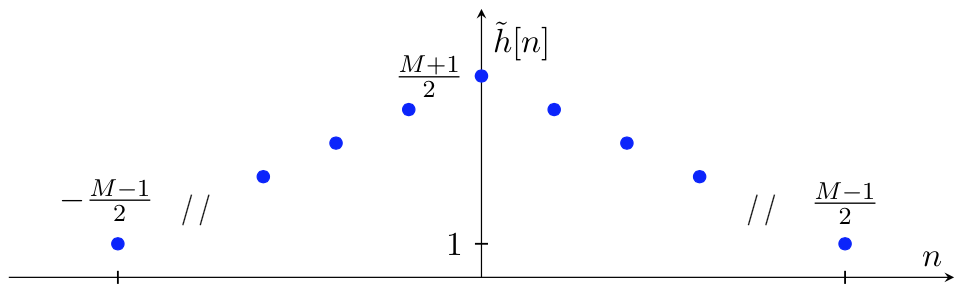
\includegraphics[width = .7\linewidth]{Filtering/NCWMAImpulseResponse.png}
\end{center}
An NCWMA Filter does \textbf{not} add any phase.\\
In general, if $H(z)$ is the transfer function of a MA filter with $M$ coefficients, then $H(z)H(z^{-1})$ is a non-causal WMA filter with $2M-1$ coefficients. 


        %!Tex root=ZF_bmicha_SaS.tex
\section{Infinite Impulse Response (IIR) Filters}
IIR filters have an LCCDE of the form
\begin{align*}
	y[n] &= \sum_{k=0}^{M-1} b_ku[n-k]-\sum_{k=1}^{N-1} a_k y[n-k]
\end{align*}
The filter order is given by $\text{max}(M-1,N-1)$ and is the size of the state in a state-space description of the system.

\subsubsection{Transfer Function and Frequency Response}
\vspace{-1em}
\begin{align*}
	H(z) &= \frac{\sum_{k=0}^{M-1}b_kz^{-k}}{1+\sum_{k=1}^{N-1}a_kz^{-k}} & H(\Omega) &= \frac{\sum_{k=0}^{M-1}b_ke^{-j\Omega k}}{1+\sum_{k=1}^{N-1}a_ke^{-j\Omega k}}
\end{align*}

\subsection{First-Order Low-Pass Filter}
First-order, low-pass, causal IIR Filters have the LCCDE
\begin{align*}
	y[n] &= \alpha y[n-1] + (1-\alpha)u[n]
\end{align*}
and are stable if $0\leq \alpha < 1$.

\subsubsection{Transfer Function and Frequency Response}
\vspace{-1em}
\begin{align*}
	H(z) &= \frac{1-\alpha}{1-\alpha z^{-1}} & H(\Omega) &= \frac{1-\alpha}{1-\alpha e^{-j\Omega}}
\end{align*}

\subsubsection{Decay Time}
Time $T_0$ to reach the value $e^{-1}$. Assume $y[0] = 1$ and $u[n] = 0$.
\begin{align*}
	\alpha &= e^{-\frac{T_s}{T_0}} \approx 1-\frac{T_s}{T_0} \quad T_0\gg T_s
\end{align*}
Longer Decay Time results in faster magnitude decrease w.r.t. frequency.

\subsection{Butterworth Filter Design (Low-Pass)}
The CT frequency response with cutoff frequency at 1 rad/sec
\begin{align*}
	R(\omega) &= \frac{1}{\sqrt{1+\omega^{2K}}}
\end{align*}
where $K$ is the order of the filter, serves as starting point.

\subsubsection{Transfer Function}
The only stable TF that has the above frequency response is
\begin{align*}
	H(s) &= \left(\prod\limits_{k = 1}^{K} (s-s_k)\right)^{-1} & s_k &= e^{\frac{j(2k + K -1)\pi}{2K}}
\end{align*}

\subsubsection{Cutoff Frequency Specification}
Get desired cutoff frequency $\omega_c$ by substitution:
\begin{align*}
	s \to \frac{s}{\omega_c}
\end{align*}

\subsubsection{Second-Order Butterworth Low-Pass Filter}
A second-order ($K=2$) Butterworth filter yields
\begin{align*}
	s_1 &= e^{j 3\pi/4} = \frac{-1+j}{\sqrt{2}} & s_2 &= e^{j 5 \pi/4} = \frac{-1-j}{\sqrt{2}}
\end{align*}
\begin{align*}
	H(s) &= \frac{\omega_c^2}{s^2+\sqrt{2} \omega_c s + \omega_c^2}
\end{align*}
    \section{Applied-Concepts}
        % Various filter designs are achieved by transforming low-pass filters with appropriate transformations, applicable in CT or DT.

\subsection{Median Filter}
	The median filter of even order $M$ is defined as
	\begin{align*}
		y[n] &= \mathop{\text{median}}(u[n-M/2], \hdots, u[n],\hdots, u[n+M/2])
	\end{align*}

\subsection{High-Pass Filter Design}
	\subsubsection{CT}
		\textbf{Goal:} High-Pass with cutoff frequency $\omega_c$\\
		1. Design low-pass $H_\text{LP}(s)$ with cutoff frequency $1/\omega_c$.\\
		2. $H_\text{HP}(s) = H_\text{LP}(s^{-1})$
		% Given a desired cutoff frequency $\omega_c$ for a high-pass filter, first design a low-pass filter $H_\text{LP}(s)$ with cutoff frequency $1/\omega_c$, and then calculate the transfer function of the corresponding high-pass filter as $H_\text{HP}(s) = H_\text{LP}(s^{-1})$

	\subsubsection{DT}
		\textbf{Goal:} High-Pass with cutoff frequency $\Omega_c$\\
		1. Design low-pass $H_\text{LP}(z)$ with cutoff frequency $\pi - \Omega_c$.\\
		2. $H_\text{HP}(z) = H_\text{LP}(-z)$
		% Given a desired cutoff frequency $\Omega_c$ for a high-pass filter, first design a low-pass filter $H_\text{LP}(z)$ with cutoff frequency at $\pi-\Omega_c$ and calculate the transfer function of the corresponding high-pass filter as $H_\text{HP}(z) = H_\text{LP}(-z)$.

\subsection{Band-Pass Filter Design}
	\subsubsection{CT  \texorpdfstring{\hfill $\omega_0 \ll \omega_1$}{}}
		% \textbf{Goal:} Band-Pass with corner frequencies $\omega_0 \ll \omega_1$\\
		% Design $H_\text{LP}(s)$ and $H_\text{HP}(s)$ with $\omega_0$ and $\omega_1$ respectively.
		\vspace{-0.5em}$$H_\text{BP}(s) = H_\text{LP}(s) \cdot H_\text{HP}(s)$$
	\subsubsection{CT}
		\textbf{Goal:} Band-Pass with corner frequencies $\omega_0 < \omega_1$\\
		1. Design low-pass filter $H_\text{LP}(s)$ with $\omega_c = \omega_1-\omega_0$.\\
		2. Transform $H_\text{LP}(s)$ using:
		% In order to obtain a band-pass with corner frequencies $\omega_0 < \omega_1$, first design a low-pass filter $H_\text{LP}(s)$ with cutoff frequency $\omega_c = \omega_1-\omega_0$ and transform it using the transformation
		\vspace{-0.5em}
		\begin{align*}
			s \to \frac{s^2+\omega_0\omega_1}{s}
		\end{align*}

\subsection{Band-Stop Filter Design}
	\subsubsection{CT \texorpdfstring{\hfill $\omega_0 \ll \omega_1$}{w0 << w1}}
		% \textbf{Assumption:} $\omega_0 \ll \omega_1$\\ 
		% \textbf{Goal:} Band-Stop with corner frequencies $\omega_0 \ll \omega_1$\\
		% 1. Design low-pass $H_\text{LP}(s)$ with cutoff frequency $\omega_0$.\\ 
		% 2. Design high-pass $H_\text{HP}(s)$ with cutoff frequency $\omega_1$.\\ 
		% Design $H_\text{LP}(s)$ and $H_\text{HP}(s)$ with $\omega_0$ and $\omega_1$ respectively.
		\vspace{-0.5em}$$H_\text{BS}(s) = H_\text{LP}(s) + H_\text{HP}(s)$$
		% Provided that $\omega_1\gg\omega_0$, design a low-pass filter $H_\text{LP}(s)$ at cutoff frequency $\omega_0$ and a high-pass filter $H_\text{HP}(s)$ at cutoff frequency $\omega_1$ and add them together to obtain a band-stop filter $H_\text{BS}(s) = H_\text{LP}(s) + H_\text{HP}(s)$.
	\subsubsection{CT}
		\textbf{Goal:} Band-Stop with corner frequencies $\omega_0 < \omega_1$\\
		1. Design low-pass filter $H_\text{LP}(s)$ with $\omega_c = 1/(\omega_1-\omega_0)$.\\
		2. Transform $H_\text{LP}(s)$ using:
		% In order to obtain a band-pass with corner frequencies $\omega_0 < \omega_1$, first design a low-pass filter $H_\text{LP}(s)$ with cutoff frequency $\omega_c = \omega_1-\omega_0$ and transform it using the transformation
		\vspace{-0.5em}
		\begin{align*}
			s \to \frac{s}{s^2+\omega_0\omega_1}
		\end{align*}
	\subsubsection{Second Order Notch Filter}
		% Notch filters are band-stop filters with a very narrow stop band.
		\vspace{-1em}
		\begin{align*}
			H_\text{NO}(s) &= \frac{s^2 + \omega_c^2}{s^2+\sqrt{2} \omega_c s + \omega_c^2}
		\end{align*}

\subsection{Bilinear Transform (BT)}
	The BT converts CT to DT filter and vice versa.
	\begin{align*}
		s = \frac{2}{T_s}\left(\frac{z-1}{z+1}\right) && z = \frac{1+s\frac{T_s}{2}}{1-s\frac{T_s}{2}}
	\end{align*}
	Maps s-plane im. axis to z-plane unit circle. (Infinities at $-1$)\\
	\textbf{BT frequency mapping}: \hfill 
	$\omega \in (-\infty,\infty) \rightarrow \Omega \in (-\pi , \pi)$
	\begin{align*}
		\Omega = 2\arctan\left(\omega\frac{T_s}{2}\right) \underbrace{\approx \omega T_s}_{\omega T_s \lesssim 0.5}
	\end{align*}
	% It conserves stability and maps every point of the frequency response of the CT filter to a corresponding point of the frequency response of the DT filter, meaning that it doesn't alter gain and phase, only shifts the frequency of the feature.
	\subsubsection{Frequency Prewarping}
		% The bilinear transform preserves stability and maps the imaginary axis in the $s$-plane to the unit circle in the $z$-plane by compressing the CT frequencies $-\infty < \omega < \infty$ to DT frequencies $-\pi < \Omega < \pi$. We can calculate the mapping using
		
		BT frequency mapping only yields desired cutoff frequencies for small $\omega$. $\rightarrow$ Prewarp CT frequencies before applying BT.
		\begin{enumerate}
			\item Let $\omega_c$ be the desired CT corner frequency.
			\item $\bar{\omega}_c = \frac{2}{T_s} \tan\left(\frac{\omega_c T_s}{2}\right)$
			\item Design CT filter with $\bar{\omega}_c$ and obtain $H(s)$.
			\item Apply BT to obtain DT filter $H(z)$ with $\Omega_c \approx \omega_c$.
		\end{enumerate}
    \section{System Identification}
        %This course focuses on the black-box identification of a causal LTI system G in the frequency domain.
\tikzstyle{block} = [draw, rectangle, fill = white, minimum height=2em, minimum width=3em]
\tikzstyle{dynblock} = [draw, rectangle, fill = white, minimum height=2em, minimum width=3em, drop shadow = {black, opacity = 1, shadow xshift = 1pt, shadow yshift = -1pt}]
\tikzstyle{smallblock} = [draw, rectangle, minimum height=2em, minimum width=2em]
\tikzstyle{integrator} = [draw, rectangle, minimum height=2em, minimum width=2em, label = {center:$\int$}]
\tikzstyle{sum} = [draw, circle, node distance=1cm]
\tikzstyle{input} = [coordinate]
\tikzstyle{output} = [coordinate]
\tikzstyle{feedback} = [coordinate]
\tikzstyle{dist} = [coordinate]
\tikzstyle{coord} = [coordinate]
\tikzstyle{pinstyle} = [pin edge={to-,thin,black}]
\begin{center}
    \resizebox{!}{3.6em}{%
        \begin{tikzpicture}[auto, node distance = 2cm, >=latex',place/.style={rectangle,draw=black,thick}]
            \node[input] (input) {};
            \node[sum, right = .9cm of input] (sum1) {};
            \node[block, right = .9cm of sum1] (G) {G};
            \node[sum, right = .9cm of G] (sum2) {};
            \node[output, right = .9cm of sum2] (output) {};
            \node[coord, above = .5cm of sum1] (ud) {};
            \node[coord, above = .5cm of sum2] (yd) {};

            \draw[->] (input) --node[below]{$u_e$} (sum1);
            \draw[->] (sum1) -- (G);
            \draw[->] (G) --node[below]{$y$} (sum2);
            \draw[->] (sum2) --node[below]{$y_m$} (output);
            \draw[->] (ud) --node[right]{$u_d$} (sum1);
            \draw[->] (yd) --node[right]{$y_d$} (sum2);
        \end{tikzpicture}
    }

\end{center}
\vspace*{-.5em}
\begin{itemize}
    \item		$u_e$ is a known input, G is causal, stable and LTI
    \item		$u_d$ is an unknown process noise, assumed to be white
    \item		$y_d$ is an unknown measurement noise, assumed to be white
    \item		$y_m$ is the measurement of the systems output, which is corrupted by process and measurement noise:
            \begin{align*}
                y_m &= Gu_e + y_d + Gu_d
            \end{align*}
\end{itemize}
        \subsection{Identification based on Impulse Responses}
\subsubsection{Without Noise}
In the absence of noise and with $\{u_e[n]\} = \{\delta[n]\}$ we have that
\begin{align*}
	\{y[n]\} &= \{h[n]\} & H(\Omega) &= \sum_{n=0}^{\infty} y_m[n]e^{-j\Omega n}
\end{align*}
Since most systems have an infinite impulse response, we collect $N$ pieces of data and then take the DFT:
\begin{align*}
	Y_m[k] &= \sum_{n=0}^{N-1} y_m[n] e^{-j\Omega_k n}
\end{align*}
At the discrete frequency $\Omega_k = 2\pi k/N$ where $k = 0,1,\hdots,N-1$, the frequency response estimate $\widehat{H}(\Omega_k)$ then becomes
\begin{align*}
	\widehat{H}(\Omega_k) \vcentcolon= Y_m[k] = H(\Omega_k) - \underbrace{\sum_{n=N}^{\infty}h[n]e^{-j\Omega_k n}}_{H_N(\Omega_k)}
\end{align*} 
Note that the error $H_N(\Omega_k) \to 0$ as $N\to\infty$ since G is stable.

\subsubsection{With Noise}
Using an impulse as input yields unsatisfactory results if noise is present since the mean squared error of the estimate approaches infinity as the length of the sample increases.

        \subsection{Identification using Sinusoidal Inputs}
Consider the case where measurement noise corrupts the output
\begin{align*}
	y_m &= Gu_e+y_d
\end{align*}
Let $u_e[n] = \textrm{exp}(j (2\pi / N) nl)$ for $n = 0,1,\hdots,N_T+N-1$, with $l$ integer, be a sinusoid with frequency $\Omega_l = 2\pi l/N$, let $y_e = Gu_e$, and let $N_T$ be sufficiently large such that the transient has decayed adequately. Since G is stable and $u_e$ is an eigenfunction of any LTI system
\begin{align*}
	y_e[n] = H(\Omega_l)u_e[n] + e_e[n], \qquad n\geq N_T
\end{align*}
where, for a fixed value of $N$, $e_e[n] \to 0$ as $N_T\to \infty$. Therefore the transient approaches $0$ and the output of the system converges to a shifted and scaled version of the input sinusoid.

\subsubsection{Frequency Response}
Taking the DFT of $y_e, e_e$ and $u_e$ yields
\begin{align*}
	Y_e[l] = H(\Omega_l) U_e[l] + E_e[l]
\end{align*}
where $E_e[l] \to 0$ as $N_T\to \infty$. Note that $U_e[l] = N$ since all the energy is concentrated at one frequency. The frequency response can be estimated
\begin{align*}
	\widehat{H}(\Omega_l) \vcentcolon= \frac{Y_m[l]}{U_e[l]} = H(\Omega_l) + \frac{E_e[l]}{N} + \frac{Y_d[l]}{N}
\end{align*}
where 
\begin{align*}
	Y_m[l] &= \hspace*{-1em}\sum_{n=N_T}^{N_T+N-1}\hspace*{-1em}y_m[n]e^{-j\frac{2\pi}{N}ln} & Y_d[l] &= \hspace*{-1em}\sum_{n=N_T}^{N_T+N-1}\hspace*{-1em}y_d[n]e^{-j\frac{2\pi}{N}ln}
\end{align*}
The same results apply to closed loop systems.

        \subsection{Identification of the Transfer Function}
%After estimating the frequency response at a number of distinct frequencies $\Omega_l$, the transfer function of the system can be identified.
Given the design parameters $A$ and $B$ (number of respective coefficients) one can identify the unknown parameters $a_k$ and $b_k$ of the system's transfer function
\begin{align*}
	H(z) &= \frac{\sum_{k=0}^{B-1}b_kz^{-k}}{1+\sum_{k=1}^{A-1}a_kz^{-k}} & H(\Omega) = \frac{\sum_{k=0}^{B-1}b_ke^{-j\Omega k}}{1+\sum_{k=1}^{A-1}a_ke^{-j\Omega k}}
\end{align*}
which results in a system of $2L$ equations
\begin{align*}
	R_l[\cos(\theta_l) + a_1\cos(\theta_l-\Omega_l) + \hdots + a_{A-1}\cos(\theta_l-(A-1)\Omega_l)] \\ =b_0 + b_1 \cos(\Omega_l) + \hdots + b_{B-1}\cos((B-1)\Omega_l) \\
	R_l[\sin(\theta_l) + a_1\sin(\theta_l-\Omega_l) + \hdots + a_{A-1}\sin(\theta_l-(A-1)\Omega_l)] \\ =-b_1 \sin(\Omega_l) - \hdots - b_{B-1}\sin((B-1)\Omega_l)
\end{align*}
This system of equations can be converted to the least squares problem of minimizing
\begin{align*}
	(F\Theta - G)^\top (F\Theta - G)
\end{align*}
where $\Theta = [a_1\quad a_2\quad\hdots\quad a_{A-1} \quad b_0 \quad b_1 \quad\hdots \quad b_{B-1}]^\top$. The LS solution yields the estimated coefficients $\Theta^*$. 
\begin{align*}
	\Theta^* &= (F^\top F)^{-1} F^\top G & \text{$F$ must have full rank}
\end{align*}

% \subsubsection{Experimental Procedure}
% \begin{enumerate}
% 	\item		Set $u_e[n] = A\cos(\Omega_ln)$ for $n = 0,\hdots,N_T+N-1$, where $N_T$ is chosen sufficiently large and $A$ scales the input such that nonlinearities are not stimulated. 
% 	\item		Take the DFT of $u_e$ and $y_m$ in the time period $n = N_T,\hdots,N_T+N-1$.
% 	\item		The frequency response estimate at the frequency $\Omega_l$ is then given by
% 			\begin{align*}
% 				\widehat{H}(\Omega_l) \vcentcolon= \frac{Y_m[l]}{U_e[l]}
% 			\end{align*}
% 	\item		Repeat this for the frequencies of interest by picking the appropriate integer $l$.
% \end{enumerate}
% Note that because the system is real, we only need to identify the frequency response for $0 \leq \Omega \leq \pi$ as we have $H(-\Omega) = H^*(\Omega)$. Therefore pick $l\in(0,(N-1)/2)$ if $N$ is odd, $l \in (0,N/2)$ if $N$ is even.

\end{document}